\documentclass[11pt,aspectratio=43]{beamer}
\usepackage[utf8]{inputenc}
\usepackage{amsmath, amsfonts, amssymb, amsthm}
\usepackage[T1]{fontenc}
\usepackage{lmodern}
\usepackage{xcolor}
\usepackage{setspace}
\usepackage{booktabs}
\usepackage{multirow}
\usepackage{graphicx}
\usepackage{tikz}
% \usetikzlibrary{decorations}
\usetikzlibrary{decorations.pathreplacing}
\usepackage{ulem}
\usepackage{hyperref}
\usepackage{booktabs}
\usepackage{babel}
\usepackage{makecell}
\usepackage[para,online,flushleft]{threeparttable}
\usepackage{pdfpages}
\usepackage{tcolorbox}
\usepackage{bm}
\usepackage{appendixnumberbeamer}
\usepackage{natbib}
\usepackage{caption}
\captionsetup[figure]{labelformat=empty}% redefines the caption setup of the figures environment in the beamer class.
\usetheme[compress]{Boadilla}
\usecolortheme{default}
\useoutertheme{miniframes}
\usefonttheme[onlymath]{serif}

\newcommand{\jump}[2]{\hyperlink{#1}{\beamerbutton{#2}}}
\newcommand{\orange}[1]{\textcolor{orange}{#1}}
\newcommand{\red}[1]{\textcolor{red}{#1}}

\setbeamertemplate{itemize item}{\raisebox{0.1em}{\scalebox{0.7}{$\blacksquare$}}}
\setbeamertemplate{itemize subitem}[circle]
\setbeamertemplate{itemize subsubitem}{--}
\setbeamercolor{itemize item}{fg=black}
\setbeamercolor{itemize subitem}{fg=black}
\setbeamercolor{itemize subsubitem}{fg=black}
\setbeamercolor{item projected}{bg=darkgray,fg=white}
\definecolor{blue}{rgb}{0.2, 0.2, 0.7}
\setbeamercolor{alerted text}{fg=blue}
\setbeamertemplate{enumerate items}[circle]


\setbeamertemplate{headline}{}

%==========================================
\let\olditemize=\itemize
\let\endolditemize=\enditemize
\renewenvironment{itemize}{\olditemize \itemsep1em}{\endolditemize}
\let\oldenumerate=\enumerate
\let\endoldenumerate=\endenumerate
\renewenvironment{enumerate}{\oldenumerate \itemsep1em}{ \endoldenumerate}

\DeclareMathOperator*{\argmax}{\arg\!\max}
\DeclareMathOperator*{\E}{\mathbb{E}}
\DeclareMathOperator*{\var}{\rm Var}
\DeclareMathOperator*{\cov}{\rm Cov}

\theoremstyle{definition}
\newtheorem{assume}{Assumption}
\newtheorem{lem}{Lemma}
\newtheorem{proposition}{Proposition}
\newtheorem{thm}{Theorem}
\newtheorem{corol}{Corollary}

\begin{document}
    \title[Lecture 3]{Lecture 3 \\ Business Cycle Measurement}
    \author[Hui-Jun Chen]{Hui-Jun Chen}
    \institute[OSU]{The Ohio State University}
    % \date{\today}
    \date{\today}
    \setbeamertemplate{navigation symbols}{}
    \setstretch{1.2}

%-------------------------------------------------------
{
%	\usebackgroundtemplate{\includegraphics[width=1\paperwidth]{../EveningSky_cropped_edit43_bright.jpg}}
    \begin{frame}
% \vspace{3em}
        \centering
%		{\footnotesize 	ECON 4002 Intermediate Macroeconomic Theory}
        \maketitle
% \vspace{-1.5em}
% \centering
% \includegraphics[width=0.55\linewidth]{Pictures/houses.jpeg}


    \end{frame}
}

% -------------------------------------------
\setbeamertemplate{headline}
{
\setbeamercolor{section in head/foot}{fg=black, bg=white}
\vskip1em \tiny \insertsectionnavigationhorizontal{1\paperwidth}{\hspace{0.50\paperwidth}}{}
}
%------------------------------------------

\section{Math Concept}
\label{sec:Math_Concept}

\begin{frame}{Review: Trend and Cycle in Per Capital Real GDP}
\label{slide:Review__Trend_and_Cycle_in_Per_Capital_Real_GDP}
\begin{columns}
    \begin{column}{0.5\textwidth}
        \begin{figure}
            \caption{Figure 1.3: Natural log of Per Capita Real GDP and trend, 1900–2014 \\ \alert{$y = \ln(Y), trend = HPFilter(y)$}}
            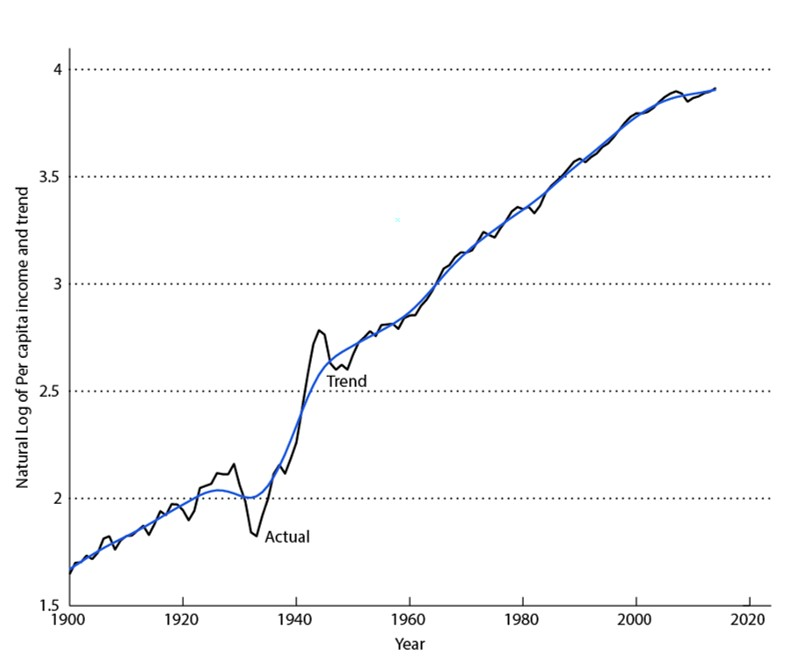
\includegraphics[width=\textwidth]{./figures/Figure1_3.jpg}
        \end{figure}
    \end{column}
    \begin{column}{0.5\textwidth}
        \begin{figure}
            \caption{Figure 1.4 Percentage Deviation from Trend in Per Capita Real GDP \\ \alert{actual - trend}}
            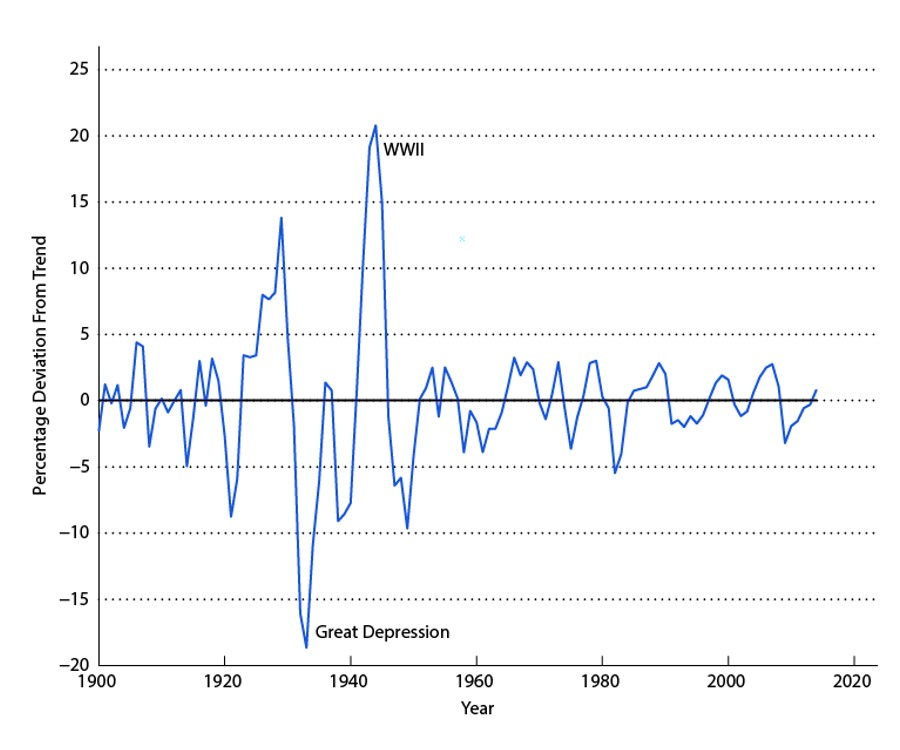
\includegraphics[width=\textwidth]{./figures/Figure1_4.jpg}
        \end{figure}
    \end{column}
\end{columns}
\begin{center}
    How do we measure the fluctuation?
\end{center}
\end{frame}

\begin{frame}{Statistical Concept to measure fluctuation}
\label{slide:Statistical_Concept}
    \begin{itemize}
        \item \textbf{mean/average} $ \bar{X} $: average level of variable $ X $
        %
        \begin{equation}
        \label{eq:average}
            \bar{X} = E( X ) \approx \frac{1}{N} \sum_{i=1}^{N} X_{i}
        ,\end{equation}
        %
        e.g. $ X = \{ 1, 2, 3, 4, 5 \} $, $ \bar{X} = \frac{1+2+3+4+5}{5} = 3 $
        \item \textbf{variance} $ \sigma_{X}^{2} $: dispersion of variable $ X $ relative to mean
        %
        \begin{equation}
        \label{eq:variance}
            \sigma_{X}^{2} = V( X ) = E[ ( X - \bar{X} )^{2} ] \approx \frac{1}{N} \sum_{i=1}^{N} [ ( X_{i} - \bar{X} )^{2} ]
        ,\end{equation}
        %
        e.g. $ \sigma_{X}^{2} = \frac{( 1-3 )^{2} + ( 2-3 )^{2} + ( 3-3 )^{2} + ( 4-3 )^{2} + ( 5-3 )^{2}}{5} = \frac{4 + 1 + 0 + 1 + 4}{5} = 2  $

        \textbf{standard deviation} is $ \sigma_{X} = \sqrt{\sigma_{X}^{2}} $.

    \end{itemize}
\end{frame}

\begin{frame}{Statistical Concept to measure fluctuation (Cont.)}
\label{slide:Statistical_Concept_to_measure_fluctuation__Cont__}
    \begin{itemize}
        \item \textbf{covariance} $ \sigma_{XY} $: dispersion of variable $ X $ ``associates'' with $ Y $.
        %
        \begin{equation}
        \label{eq:covariance}
            \sigma_{XY}
                = E[ ( X - \bar{X} ) ( Y - \bar{Y} ) ]
                \approx \frac{1}{N} \sum_{i=1}^{N} [ ( X_{i} - \bar{X} ) ( Y_{i} - \bar{Y} ) ]
        ,\end{equation}
        %
        e.g. $ Y = \{ 2, 3, 4, 5, 6 \} $, $ \bar{Y} = 4 $, $ \sigma_{XY}
                = \frac{( 1-3 )( 2-4 ) + ( 2-3 )( 3-4 ) + ( 3-3 )( 4-4 ) + ( 4-3 )( 5-4 ) + ( 5-3 )( 6-4 )}{5} = 2$
        \item \textbf{correlation} $ \rho_{XY} $: level of association between variables $ X $ and $ Y $
        %
        \begin{equation}
        \label{eq:correlation}
            \rho_{XY} = \frac{\sigma_{XY}}{\sigma_{X} \sigma_{Y}}
        ,\end{equation}
        %
        e.g. $ \rho_{XY} = \frac{2}{\sqrt{2} \times \sqrt{2}} = 1$

        $ \rho_{XY} > 0 $: $ X $ and $ Y $ move \alert{together}; $ < 0 $: move \alert{opposite} directions
    \end{itemize}
\end{frame}

\section{Measure GDP \& comove}
\label{sec:Measure_GDP____comove}

\begin{frame}{GDP Fluctuations: Definition and Measurement}
\label{slide:GDP_Fluctuations__Definition_and_Measurement}
    \begin{columns}
        \begin{column}{0.5\textwidth}
            \begin{itemize}
                \item \textbf{Business cycle}: fluctuations about trend in real GDP
                \item \textbf{Booms/Expansions}: persistent \alert{positive} deviation
                \item \textbf{Recessions}: persistent \alert{negative} deviation
                \item \textbf{Peak/Trough}: turning points on deviations
                \item \textbf{Amplitude}: size of deviations
                \item \textbf{Frequency}: \# of peaks per year
            \end{itemize}
        \end{column}
        \begin{column}{0.5\textwidth}
            \begin{figure}
                \caption{Figure 3.1 Business Cycle}
                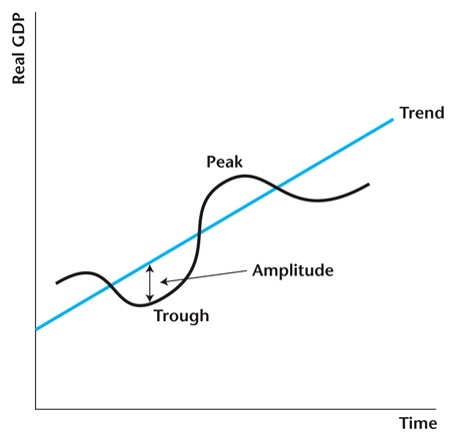
\includegraphics[width=\textwidth]{./figures/Fugre3_1.jpg}
            \end{figure}
        \end{column}
    \end{columns}
\end{frame}


\begin{frame}{Measurement on Comovement}
\label{slide:Measurement_on_Comovement}
    Three key concepts to measure comovement of variables $ X $ with GDP $ Y $:
    \begin{enumerate}
        \item \textbf{relative volatility} $ \sigma_{X} / \sigma_{Y} $: how noisy is $ X $ relative to GDP
        \begin{itemize}
            \item $ \sigma_{X} / \sigma_{Y} $ high $ \Rightarrow  $ $ X $ is noisy
        \end{itemize}
        \item \textbf{cyclicality} $ \rho_{XY} $: how does $ X $ comove with GDP?
        \begin{enumerate}
            \item \alert{procyclical}: $ \rho_{XY} > 0 $, $ X $ and GDP comove \alert{together}
            \item \alert{acyclical}: $ \rho_{XY} \approx 0 $, $ X $ and GDP not comoving
            \item \alert{countercyclical}: $ \rho_{XY} < 0 $, $ X $ and GDP move in \alert{opposite} direction
        \end{enumerate}
        \item \textbf{lead/coincident/lag}: does $ X $ predict GDP (lead), the opposite (lag) or nor (coincident)?
    \end{enumerate}
\end{frame}

\section{Visualization}
\label{sec:Visualization}

\begin{frame}{Visualization of Correlation: Scatter Plots}
\label{slide:Visualization_of_Correlation__Scatter_Plots}
    \begin{figure}
        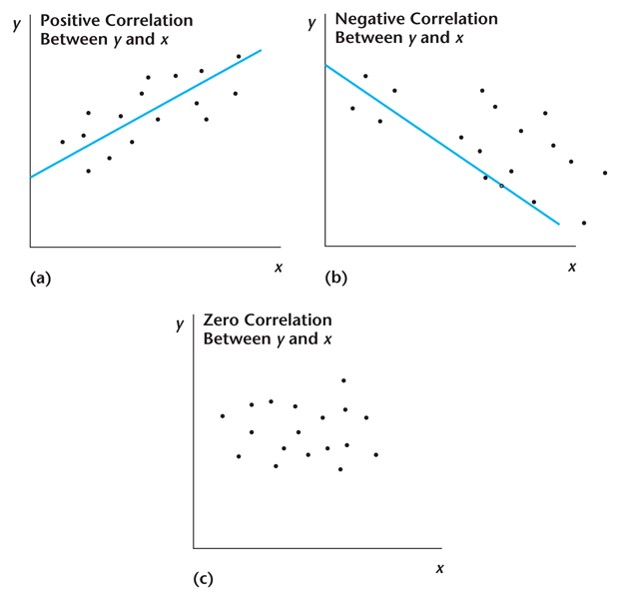
\includegraphics[width=0.65\textwidth]{./figures/Figure3_4.jpg}
    \end{figure}
\end{frame}

\begin{frame}{Visualization of Correlation: Time Series}
\label{slide:Visualization_of_Correlation__Time_Series}
    \begin{figure}
        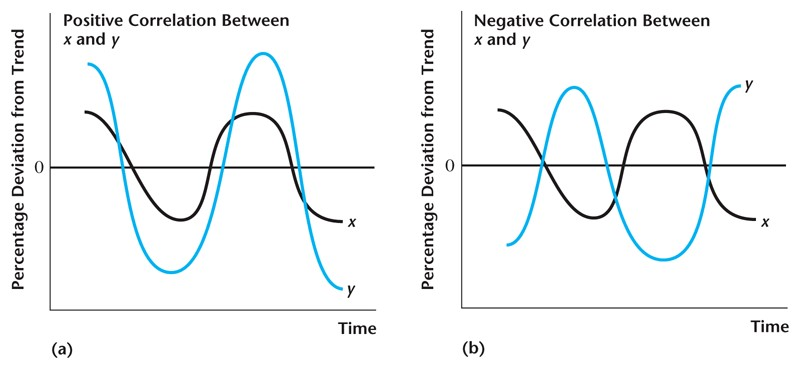
\includegraphics[width=\textwidth]{./figures/Figure3_3.jpg}
    \end{figure}
\end{frame}

\begin{frame}{Visualization of Leading and Lagging: Time Series}
\label{slide:Visualization_of_Leading_and_Lagging__Time_Series}
    \begin{figure}
        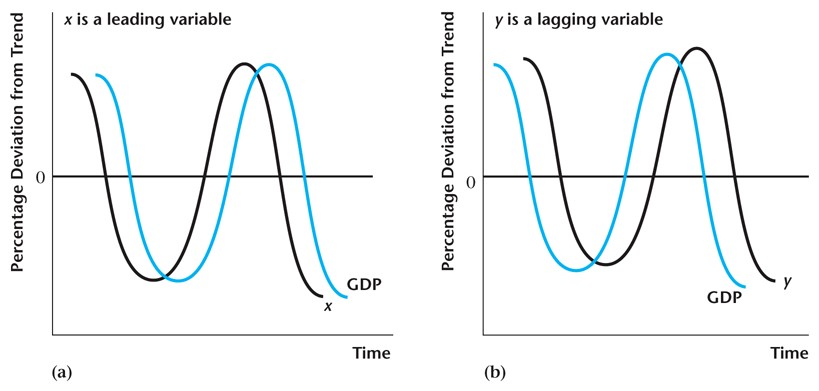
\includegraphics[width=\textwidth]{./figures/Figure3_7.jpg}
    \end{figure}
\end{frame}


\section{Data}
\label{sec:Data}

\begin{frame}{Data: Comovement of $ C $ and $ I $}
\label{slide:Data__Comovement_of___C___and___I__}

\begin{columns}
    \begin{column}{0.5\textwidth}
        \begin{figure}
            \caption{Figure 3.9 Percentage Deviations from Trend in \alert{Real Consumption} and Real GDP}
            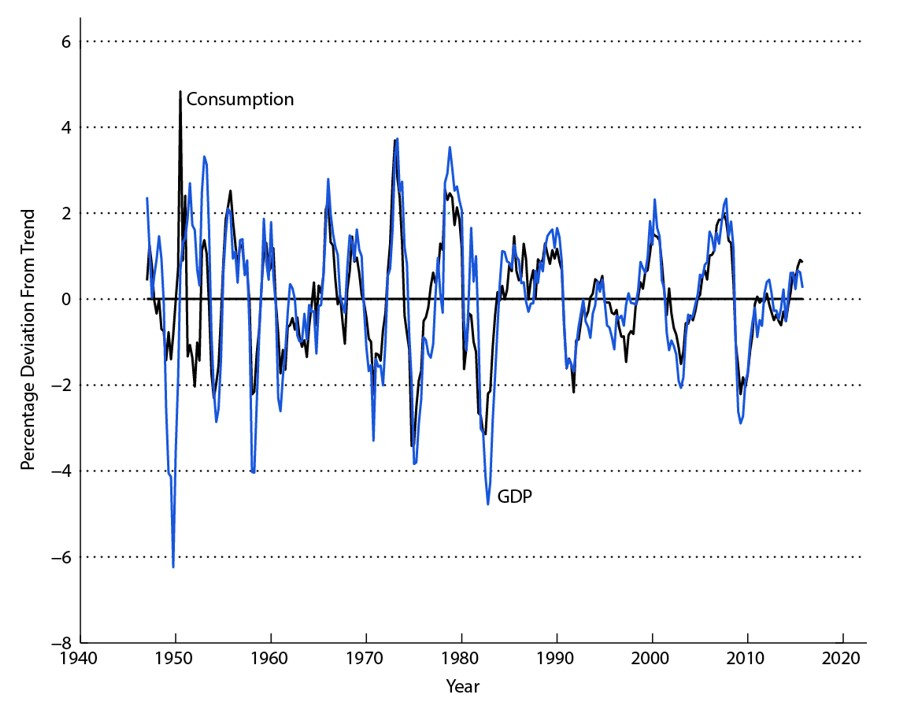
\includegraphics[width=\textwidth]{./figures/Figure3_9.jpg}
        \end{figure}
    \end{column}
    \begin{column}{0.5\textwidth}
        \begin{figure}
            \caption{Figure 3.10 Percentage Deviations from Trend in \alert{Real Investment} and Real GDP}
            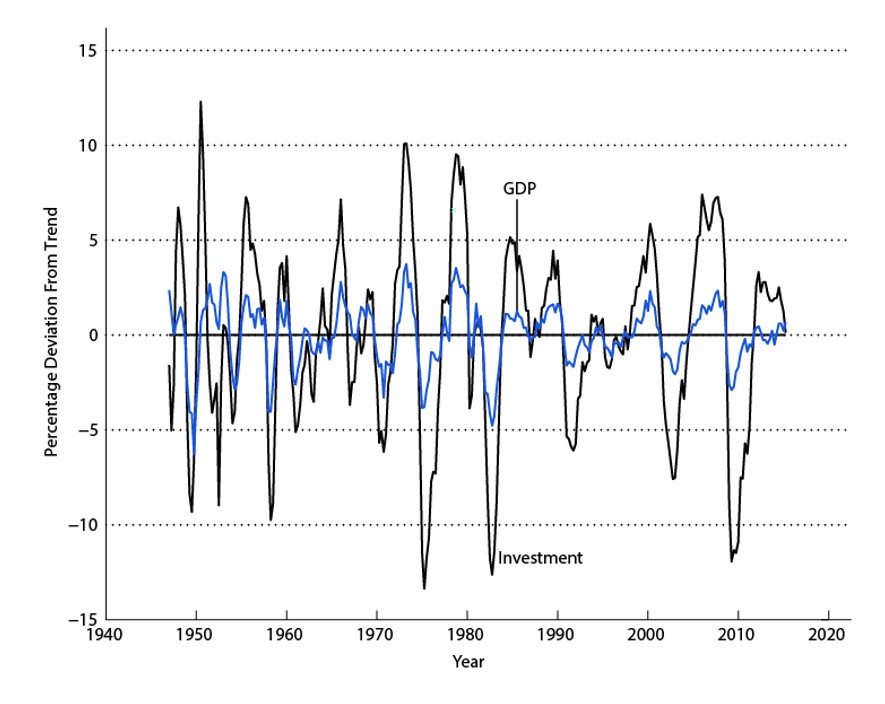
\includegraphics[width=\textwidth]{./figures/Figure3_10.jpg}
        \end{figure}
    \end{column}
\end{columns}
\end{frame}

\begin{frame}{Data: Correlation of Imports}
\label{slide:Data__Correlation_of_Imports}
    \begin{columns}
        \begin{column}{0.5\textwidth}
            \begin{figure}
                \caption{Figure 3.5  Time Series (Detrended)}
                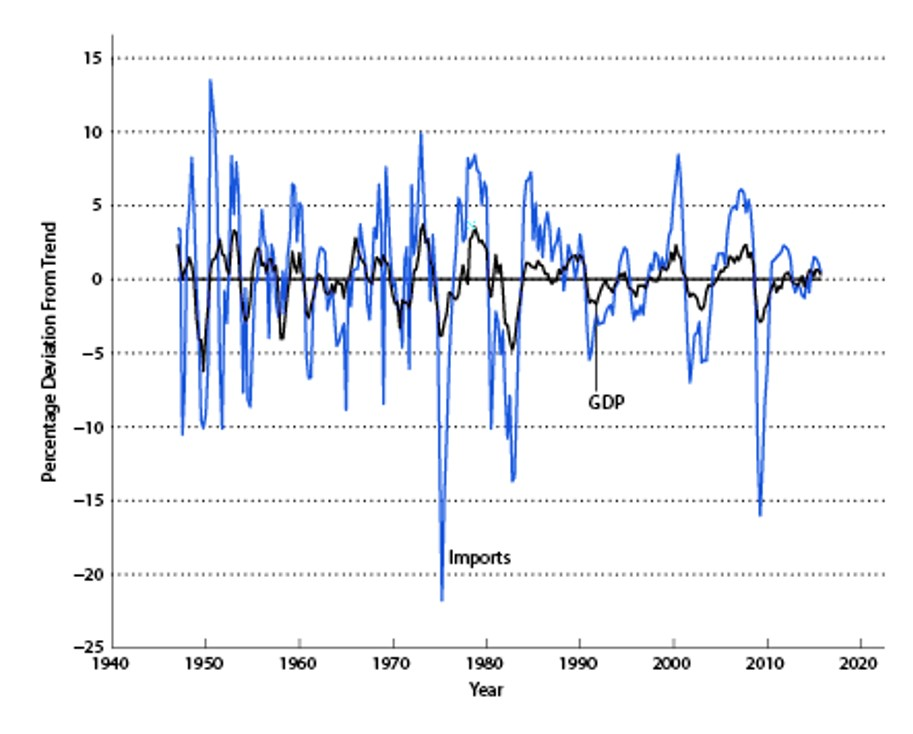
\includegraphics[width=\textwidth]{./figures/Figure3_5.jpg}
            \end{figure}
        \end{column}
        \begin{column}{0.5\textwidth}
            \begin{figure}
                \caption{Figure 3.6  Scatter Plot: Time Series}
                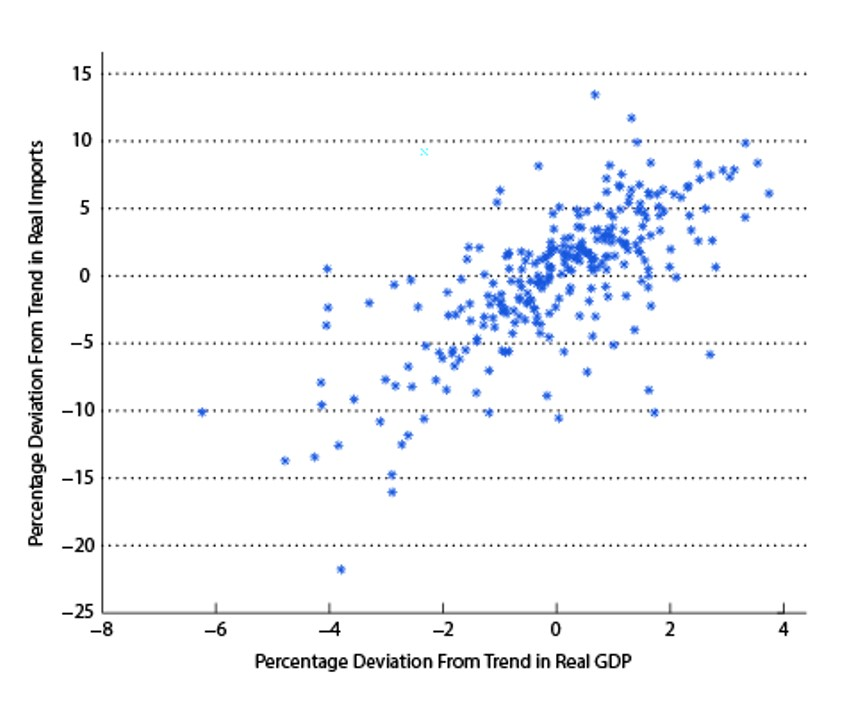
\includegraphics[width=\textwidth]{./figures/Figure3_6.jpg}
            \end{figure}
        \end{column}
    \end{columns}
\end{frame}

\begin{frame}{Data: Leading Indicator, Housing Starts}
\label{slide:Data__Leading_Indicator}
    \begin{columns}
        \begin{column}{0.5\textwidth}
            \begin{figure}
                \caption{Figure 3.8  Percentage Deviations in Real GDP and Housing Starts}
                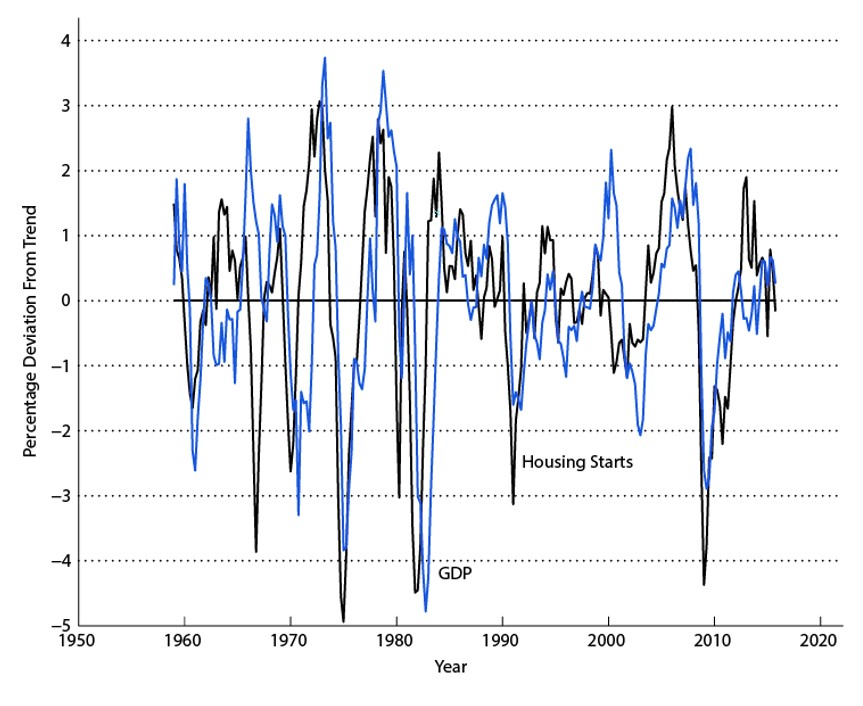
\includegraphics[width=\textwidth]{./figures/Figure3_8.jpg}
            \end{figure}
        \end{column}
        \begin{column}{0.5\textwidth}
            \begin{itemize}
                \item \textbf{Def}: the construction project is started for a private dwelling
                \item \alert{Question}: Why housing start is predicting GDP?
                \item Ans: \alert{commitment} to a quantity of residential \alert{investment}
            \end{itemize}
        \end{column}
    \end{columns}
\end{frame}

\begin{frame}{Summary}
\label{slide:Summary}
    \begin{figure}
        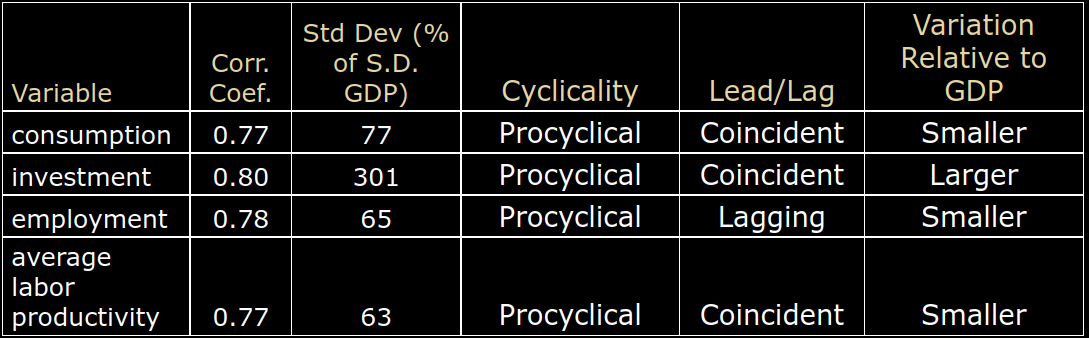
\includegraphics[width=\textwidth]{./figures/BCSummary.png}
    \end{figure}

    What about the properties of government spending? Expectation?
\end{frame}




\end{document}

